\documentclass[tikz,border=8pt]{standalone}
\begin{document}
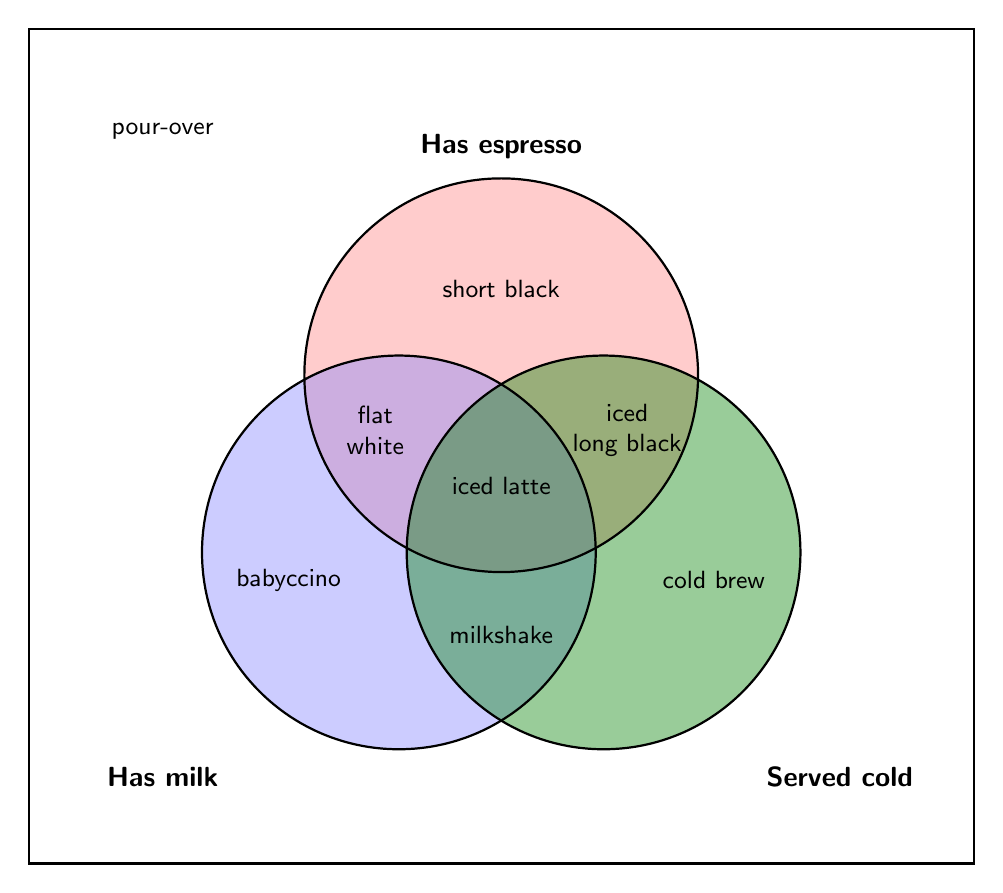
\begin{tikzpicture}[font=\sffamily\small,align=center]
\draw[thick] (-6,-4.8) rectangle (6,5.8);
\fill[red!50,opacity=.4] (0,1.4) circle (2.5);
\fill[blue!50,opacity=.4] (-1.3,-0.85) circle (2.5);
\fill[green!50!black,opacity=.4] (1.3,-0.85) circle (2.5);
\draw[thick] (0,1.4) circle (2.5);
\draw[thick] (-1.3,-0.85) circle (2.5);
\draw[thick] (1.3,-0.85) circle (2.5);
\node[font=\sffamily\bfseries] at (0,4.3) {Has espresso};
\node[font=\sffamily\bfseries] at (-4.3,-3.7) {Has milk};
\node[font=\sffamily\bfseries] at (4.3,-3.7) {Served cold};
\node at (0,2.5) {short black};
\node at (-2.7,-1.2) {babyccino};
\node at (2.7,-1.2) {cold brew};
\node at (-1.6,0.7) {flat\\white};
\node at (1.6,0.7) {iced\\long black};
\node at (0,-1.9) {milkshake};
\node at (0,0) {iced latte};
\node at (-4.3,4.5) {pour-over};
\end{tikzpicture}
\end{document}
